%%
%% Author: thompson
%% 26.10.17
%%

% Preamble
\documentclass[11pt]{article}

% Packages
\usepackage{a4wide}
\usepackage[utf8]{inputenc}
\usepackage[ngerman]{babel}
\usepackage{graphicx}

% Document
\begin{document}

\section{ISO-OSI Referenzmodel}

    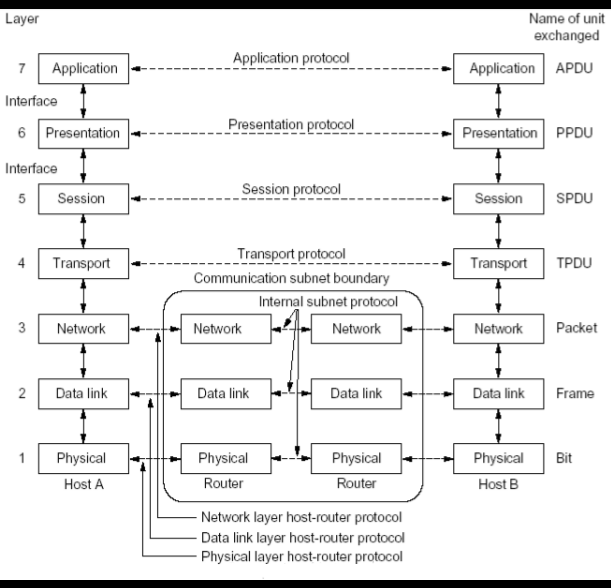
\includegraphics[width=\textwidth]{ISO_OSIReferenceModel.png}

    Das ISO-OSI Referenzmodell besteht aus verschiedenen Anwendungsschichten:
    \begin{enumerate}
        \item Physical Layer\\
        Dieser Layer beschreibt die fundamentale Netzwerkkommunikation. Datentransfer via
        physischem Layer sind reine Bitstreams.
        \item Data Link Layer\\
        Der Datenlink nutzt die Daten vom Physischen Layer und bündelt die Bits zu Frames zusammen.

        \item Network Layer
        \item Transport Layer
        \item Session Layer
        \item Presentation Layer
        \item Application Layer
    \end{enumerate}

\end{document}